\documentclass[a4paper,10pt]{article}
\usepackage[utf8]{inputenc}
\usepackage[ngerman]{babel}
\usepackage{a4wide}
\usepackage{tabularx}
\usepackage{amsmath}
\usepackage{amssymb}
\usepackage{url}
\usepackage{tikz,pgfplots}
\usepackage[section]{placeins} 
\usetikzlibrary{fpu}
%%\usepackage[pdf]{pstricks}
\setlength{\parindent}{0pt}

%opening
\title{Grundlagen der Kommunikationstechnik}
\author{Julian-B. Scholle}

\begin{document}

\maketitle

\begin{abstract}

\end{abstract}

\section{Einleitung}

Kommunikation ist die Übertragung von Informationen zwischen 2 oder mehreren Stellen. 

\subsection{Die Kommunikationskette}
Beispiel: Das Telefonieren\\

\begin{tabularx}{\textwidth}{rlXl}
1   & Informationsquelle &  \^=  & Gehirn  \\ 
2   & 1. Wandler &  \^=  & Mund + Stimmensystem $\rightarrow$ akustisches Signal  \\ 
3   & 2. Wandler &  \^=  & Mikrofon $\rightarrow$ elektrisches Signal  \\ 
4   & Signal(a) &  \^=  & Strom und Spannung am Ausgang des Mikrofons  \\ 
5   & Sender &  \^=  & das Telefongerät  \\ 
6   & Signal(b) &  \^=  & EM-Welle für Mobilfunk oder Strom und Spannung im Festnetz  \\ 
7   & Übertragungskanal &  \^=  & Funkkanal(Mobilfunk) oder Telefonleitung(Festnetz)  \\ 
8   & Empfänger &  \^=  & das Telefongerät  \\ 
9   & Signal(c) &  \^=  & Strom und Spannung am Eingang des Lautsprechers  \\ 
10   & 1. Wandler &  \^=  & der Lautsprecher $\rightarrow$ akustisches Signal  \\ 
11   & 2. Wandler &  \^=  & Das Ohr und das Hörsystem  \\ 
12   & Informationssenke &  \^=  & Gehirn 
\end{tabularx}

\subsection{Die Information}
Die Information ist die Ordnung von Informationsträgern. Sie ist vervielfachbar.\\
zum Beispiel:\\\\
\begin{tabularx}{\textwidth}{lX}
  Text & Informationsträger sind die Buchstaben. Die Ordnung dieser Buchstaben ist die Information. \\
  Sprache & Informationsträger sind die Laute. Die Ordnung der Laute ist die Information \\
  Bilder und Bildsequenzen & Informationsträger sind die Pixel. Die Ordnung dieser Pixel ist die Information\\
\end{tabularx}

\subsection{Der Wandler}
Der Wandler ist eine Schnittstelle (Hardware) die ein Signal (Zeitabhängiger physikalischer Vorgang, der Energie enthält) erzeugt, das Informationen trägt.
Signale sind deshalb Informationsträger. Der zeitliche Verlauf ist die Ordnung, welche die Information darstellt.\\
In diesem Zusammenhang ist der Mund und das Stimmensystem ein Wandler. Hier wird ein akustisches Signal erzeugt, dessen Form (d.h. sein zeitlicher Verlauf) die Information darstellt.
Das Mikrofon und die Kamera sind ebenfalls Wandler, beide erzeugen ein elektrisches Signal dessen zeitlicher Verlauf die Information darstellt(trägt).


\subsection{Das Signal}
Signale sind Informationsträger, die in der Lage sind, aufgeprägte Informationen zu übertragen.
Zum Beispiel in form von Strom und Spannung. Die Medien sind dabei messbar und verfügen über Energie.

Die Informationstragenden Signale lassen sich wie folgt Klassifizieren:\\

\subsubsection{Analog}
Das Signal ist ein kontinuierlicher Vorgang z.B. ein Akustisches Signal.

\begin{figure}[!htb]
\centering
\begin{tikzpicture}
	%Raster zeichnen
	\draw [color=gray!30]  [step=5mm] (0,0) grid (7,3);
	% Achsen zeichnen
	\draw[->,thick] (0,0) -- (7.5,0) node[right] {$t$};
	\draw[->,thick] (0,0) -- (0,3.3) node[above] {$S(t)$};
	% Achsen beschriften
	%\foreach \x in {0,1,2,3} \draw (\x,-.2) -- (\x,0) node[below=4pt] {$\scriptstyle\x$};
	%\foreach \y in {0,1,2,3} \draw (-.1,\y) -- (.1,\y) node[left=4pt] {$\scriptstyle\y$};
	 \draw (0,1) sin(1,2) cos(2,1) sin(3,0) cos(4,1) sin(5,2) cos(6,1) sin(7,0);
	%\draw [color=red] plot [smooth] coordinates{(0,1) (1,2) (2,1) (3,2) (4,1)(5,2)(6,1)(7,2)};
\end{tikzpicture}
\caption{analoges Signal}%
\label{analog}
\end{figure}




\subsubsection{Digital}

Das Signal ist eine Sequenz von einzelnen(zeitlich kompakten) Einheiten(Symbolen)

\begin{figure}[!htb]
\centering
\begin{tikzpicture}
	%Raster zeichnen
	\draw [color=gray!30]  [step=5mm] (0,0) grid (7,3);
	% Achsen zeichnen
	\draw[->,thick] (0,0) -- (7.5,0) node[right] {$t$};
	\draw[->,thick] (0,0) -- (0,3.3) node[above] {$S(t)$};
	%graph
	\draw (0,0)--(1,0) -- (1,1) -- (2,1) -- (2,0) -- (3,0) -- (3,1.5) -- (6,1.5) -- (6,0) -- (7,0);
\end{tikzpicture}
\caption{digitales Signal}%
\label{digital}
\end{figure}


Digitale Signale, zum Beispiel Morse-Code, tragen codierte Informationen

\subsubsection{Monochromatisch}
Monochromatische Signale sind Signale mit nur einer Frequenz.
\begin{align}
  S_mc = \hat{S} \cdot cos(\omega_0t-\varphi_0)
\end{align}
 
Wie zum Beispiel die Netzspannung (Sinussignal)


 
\subsubsection{periodische Signale (nicht monochromatisch)}
Ein Signal ist periodisch wenn:
\begin{align}
   S_p(t\pm n\cdot T) = S_p(t)
\end{align}

\subsubsection{nichtperiodische Signale}
Ein Signal ist nicht periodisch wenn:
\begin{align}
   S_p(t\pm n\cdot T) \neq S_p(t)
\end{align}


\subsection{Codierung}
Ein Code ist eine Sequenz von Symbolen.\\
zum Beispiel:\\
\begin{itemize}
 \item Zahlen: Sequenz der Symbole 1,2,....,9,0
 \item Texte: Sequenz der Symbole a,b,c,...
\end{itemize}
Um die Informationen zu Codieren, und damit digitale Signale zu erzeugen, braucht man ein Codierungsverfaren(Sogenannte Quellencodierung),
das die Information auf Sequenzen von Symbolen abbildet.
zum Beispiel:\\
\begin{itemize}
 \item Das Gehirn bildet Begriffe,Gefühle,Eindrücke,... auf Wörter ab. Diese sind Sequenzen von Buchstaben (oder Lauten)
 \item Der Morse-Code
\end{itemize}

\subsection{Der Sender und der Empfänger}
Die Aufgabe des Senders ist die Erzeugung eines Signals(b), das die gleiche Information wie Signal(a)
enthält, aber mehr geeignet für die Übertragung durch den Kanal ist.


Die Aufgabe des Empfängers ist die Erzeugung eines Signals(s) das die gleiche Information wie Signal(b)
enthält, aber mehr geeignet ist für den Wandler an der Empfängerseite.

\newpage
\section{Der Übertragungskanal}

Übertragungskanäle werden in dratgebundene und Dratlose gruppiert:

\subsection{Drahtgebunden}


\subsubsection{Kupferkabel / Telefonkabel}

\begin{figure}[!htb]
\centering
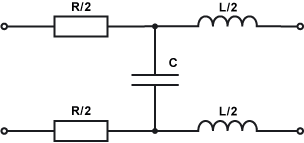
\includegraphics[scale=0.5]{Kupferkabel.png}\\
\caption{Ersatzschaltbild eines Leiters}%
\label{kupferkabel}
\end{figure}

Die Schaltung [\ref{kupferkabel}] ist das Ersatzschaltbild einer gleichmäßig aufgebauten (homogenen) Leitung. Jede 2-adrige Leitung entspricht diesem Ersatzschaltbild.
Sie ist nicht nur mit einem Widerstand, sondern auch mit einer Induktivität und Kapazität behaftet. Demzufolge ist dieser Leitungsvierpol frequenzabhängig
und zu allem Überfluss auch noch ein Schwingkreis. Zusätzlich werden die elektrischen Eigenschaften durch die Leitungskonstruktion beeinflusst (Verseilungsart, Feuchtigkeit, etc.).
\paragraph{Probleme}
\begin{itemize}
  \item Übersprechen zwischen den Leitungen
  \item Signaldämpfung (Signalverluste) durch die Leitungslänge
  \item Leitungscharakteristik ist immer anders
\end{itemize}



\subsubsection{Koaxialkabel}
\begin{figure}[!htb]
\centering
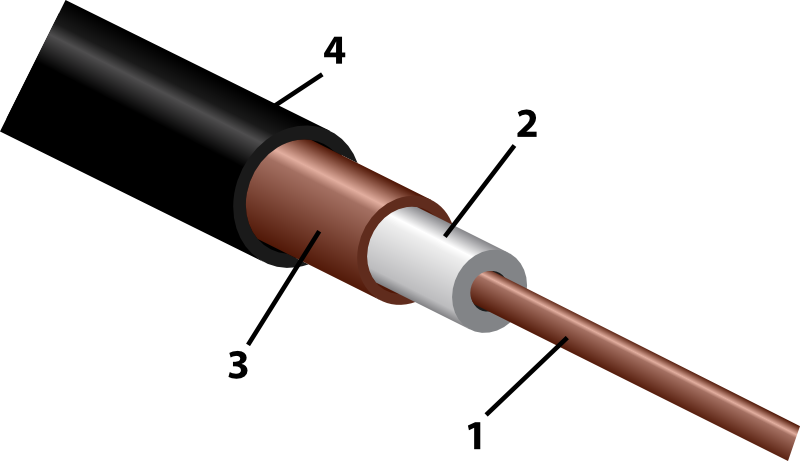
\includegraphics[scale=0.5]{Coaxial.png}\\
\caption{schematischer Aufbau eines Koaxialkabels}%
\label{coaxialkabel}
\end{figure}

Das Koaxialkabel [\ref{coaxialkabel}] ist ein unsymmetrisches Kabel. Bei der Übertragung von digitalen Signalen über ein Koaxialkabel (BNC) wird ein Potentialunterschied zwischen 
Innenleiter (Kern) und dem, als Bezugserde dienenden, Außenleiter erzeugt. Der Außenleiter wirkt als Antenne. Er strahlt elektromagnetische Strahlen ab. 
Zusätzlich beeinflussen Störungen von außen den Signalfluss im Innenleiter.Damit die elektrische Feldverteilung wirksam wird, muss der Außenleiter (Abschirmung,
Abschirmmantel) an Erde gelegt werden. Hierdurch sind beide Leiter gegenüber der Erde spannungsmäßig ungleich. Deshalb sind Koaxialkabel unsymmetrische Leitungen
(Paralleldrahtleitungen sind erdsymmetrisch).


\paragraph{Vorteile}
\begin{itemize}
 \item Es können keine Störspannungen durch Influenz in das Kabel gelangen.
 \item Die im Kabel fließenden Ströme erzeugen keine magnetischen Störfelder.
\end{itemize}


\paragraph{Einsatzgebiet:}Kabel/Satelliten-TV\\
\paragraph{Frequenz:}bis ca. 1Ghz\\

\subsubsection{Hohlleiter}
Ein Hohlleiter ist ein Wellenleiter für elektromagnetische Wellen vorwiegend im Zentimeter-Wellenbereich und darunter (ca. 3 GHz bis 200 GHz). Hohlleiter sind Metallrohre 
mit meist rechteckigem, kreisförmigem oder elliptischem Querschnitt, in denen sich derart hohe Frequenzen im Gegensatz zu Kabeln sehr verlustarm übertragen lassen.


\subsubsection{Lichtwellenleiter}
\begin{figure}[!htb]
\centering
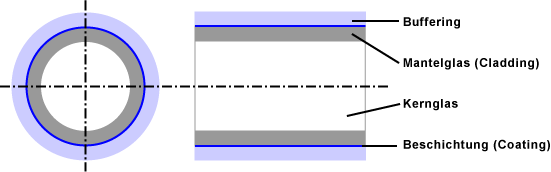
\includegraphics[scale=0.5]{LWL.png}\\
\caption{schematischer Aufbau eines Lichtwellenleiters}%
\label{lichtwellenleiter}
\end{figure}

Lichtwellenleiter [\ref{lichtwellenleiter}] übertragen Daten in Form von Licht bzw. Lichtsignalen über weite Strecken. Während elektrischen Signale in Kupferleitungen
als Elektronen von einem zum anderen Ende wandern, übernehmen in Lichtwellenleitern die Photonen diese Aufgabe.

Durch Lichtwellenleiter können optische Signale ohne Verstärker große Entfernungen überbrücken. Trotz weiter Strecken ist eine hohe Bandbreite möglich. 
Die Bandbreite auf einer einzigen Glasfaser beträgt rund 60 THz. Das macht Lichtwellenleiter zum Übertragungsmedium der Gegenwart und Zukunft. Da reicht kein Kupferkabel oder Funksystem heran.

\paragraph{Vorteile}
\begin{itemize}
 \item Lichtwellenleiter können beliebig mit anderen Versorgungsleitungen parallel verlegt werden. Es gibt keine elektromagnetischen Störeinflüsse.
 \item Wegen der optischen Übertragung existieren keine Störstrahlungen oder Masseprobleme.
 \item Entfernungsbedingte Verluste des Signals wegen Induktivitäten, Kapazitäten und Widerständen treten nicht auf.
 \item Nahezu Frequenz-unabhängige Leitungsdämpfung der Signale.
 \item Übertragungsraten sind durch mehrere Trägerwellen mit unterschiedlichen Wellenlängen (Farbspektrum) fast unbegrenzt erweiterbar.
\end{itemize}

\subsection{Dratlose}

Das Übertragungssignal ist hier eine EM-Welle, die sich durch die Atmosphäre ausbreitet.

\paragraph{Oberflächenwellen}


300KHz ($\lambda = 1000m $) bis 3MHz ($\lambda = 100m $)


%
%
%%
%%%
%%%%
%%%%%BILDER
%%%%%%
%%%%%%%
%%%%%%%%
%%%%%%%%%
%%%%%%%%%%

Hauptproblem ist hier die Antennenlänge
Antennenlänge $\geq \frac{\lambda}{10}$ 

Masten+ horizontale Dräte zwischen 10m und 100m

Am-Radio (Rundfunk \^= in alle Richtungen )

Mittelwelle 3 MHz-> 10MHz
kurze Reichweite

Kurzwelle 10MHz -> 39MHz
Lange Reichweite


TV(Richtfnk)
VHF 30MHz -> 300MHz
UHF 300MHz -> 3GHz


Mobilfunk

GSM 900MHz,1800MHz
UMTS 2400MHz

Wlan 2,4GHz/5,4 GHZ




\newpage
\section{Periodische Signale}
\subsection{Die Fourierreihe}

Periodische Signale lassen sich nach einer Fourierreihe zerlegen:

\begin{align}
 f_p(t)&=a_0+\sum_{k=1}^\infty a_k cos(k\omega t)+ \sum_{k=1}^\infty b_k sin(k\omega t)\\
 a_0 &= \frac{1}{T} \int_{t_0}^{t_0+T} f_p(t) df = Mittelwert \\
 a_k &= \frac{1}{T} \int_{t_0}^{t_0+T} f_p(t) cos(k\omega t) df \\
 b_k &= \frac{1}{T} \int_{t_0}^{t_0+T} f_p(t) sin(k\omega t) df
\end{align}

mit:\\
$b_k$ für alle $k$, falls $f$ gerade ist ,$f(-x)=f(x)$\\
$a_k$ für alle $k$, falls $f$ ungerade ist ,$f(-x)=-f(x)$\\

\subsection{Das Amplituden- und Phasen-Spektrum}

Das Amplituden [\ref{amplituden_spektrum}] - und Phasen [\ref{phasen_spektrum}] -Spektrum sind grafische Darstellungen für $|F_n|$ bzw $\varphi_n$:

\begin{figure}[!htb]
\centering
\begin{tikzpicture}[domain=-4:4]
	%Raster zeichnen
	\draw [color=gray!30]  [step=5mm] (-4,0) grid (4,3);
	% Achsen zeichnen
	\draw[->,thick] (-4,0) -- (4.5,0) node[right] {$n$};
	\draw[->] (0,0) -- (0,3.3) node[above] {$|F_n|=\widehat{F_n}$};
	%graph
	\draw [-|,thick](-2,0)--(-2,0.8) node[above] {$|F_{-2}|$};
	\draw [-|,thick](-1,0)--(-1,1.4) node[above] {$|F_{-1}|$};
	\draw [-|,thick](0,0)--(0,1) node[above] {$|F_{0}|$};
	\draw [-|,thick](1,0)--(1,1.4) node[above] {$|F_{1}|$};
	\draw [-|,thick](2,0)--(2,0.8 )node[above] {$|F_{2}|$};
	\draw [xshift=-0cm](-3 cm,1pt) -- (-3 cm,-3pt)       node[anchor=north] {$\cdots$};
	\draw [xshift=-0cm](3 cm,1pt) -- (3 cm,-3pt)       node[anchor=north] {$\cdots$};
	\foreach \x in {-2,-1,0,1,2}
        \draw [xshift=-0cm](\x cm,1pt) -- (\x cm,-3pt)
            node[anchor=north] {$\x$};

\end{tikzpicture}
\caption{Amplituden-Spektrum}
\label{amplituden_spektrum}
\end{figure}


\begin{figure}[!htb]
\centering
\begin{tikzpicture}[domain=-4:4]
	%Raster zeichnen
	\draw [color=gray!30]  [step=5mm] (-4,-3) grid (4,3);
	% Achsen zeichnen
	\draw[->,thick] (-4,0) -- (4.5,0) node[right] {$n$};
	\draw[->] (0,-3) -- (0,3.3) node[above] {$\varphi_n$:};
	%graph
	\draw [-|,thick](-2,0)--(-2,0.8) node[above] {$-\varphi_{-2}$};
	\draw [-|,thick](-1,0)--(-1,1.4) node[above] {$-\varphi_{-1}|$};

	\draw [-|,thick](1,0)--(1,-1.4) node[above] {$-\varphi_{1}$};
	\draw [-|,thick](2,0)--(2,-0.8 )node[above] {$-\varphi_{2}|$};
	\draw [xshift=-0cm](-3 cm,1pt) -- (-3 cm,-3pt)     node[anchor=north] {$\cdots$};
	\draw [xshift=-0cm](3 cm,1pt) -- (3 cm,-3pt)       node[anchor=north] {$\cdots$};
        \draw [xshift=-0cm](0 cm,1pt) -- (0 cm,-3pt)       node[anchor=north] {$\varphi_{0}$};

\end{tikzpicture}
\caption{Phasen-Spektrum}
\label{phasen_spektrum}
\end{figure}


Symmetrie: $F_{-n}=F_n*$. Dies quantisiert dass die Summe aller komplexen Phasoren null ist.\\


\begin{figure}[!htb]
\centering
\begin{tikzpicture}[y=3.34cm,x=0.318cm,domain=-15:15]
    \draw [color=gray!30] [step=3.34mm] (-15,-0.3) grid (15,1.05);
    \draw[->] (-15.3,0) -- (15.3,0) node[right] {$t[s]$};
    \draw[->] (0,-0.3) -- (0,1.1) node[above] {$S$};
    \draw [-](-2.08,0.5)--(2.08,0.5) node[above] {};
    \draw [-](-2.08,0)--(-2.08,0.5) node[above] {};
    \draw [-](2.08,0)--(2.08,0.5) node[above] {};
    

    
    \draw [|-|](2.08,-0.16)--(10.5,-0.16) node[above] {};  
    \draw [xshift=-0cm](6.29,-0.16) node[anchor=north] {$T_P$};
     \draw [|-|](6.3,-0.1)--(10.5,-0.1) node[above] {};  
    \draw [xshift=-0cm](8.4,-0.1) node[anchor=north] {$T_I$};
    
    
    \draw [-](6.3,0)--(6.3,0.5) node[above] {};  
    \draw [-](6.3,0.5)--(10.5,0.5) node[above] {};
    \draw [-](10.5,0.5)--(10.5,0) node[above] {};
    \draw [-](14.75,0)--(14.75,0.5) node[above] {};  
    \draw [-](14.75,0.5)--(15,0.5) node[above] {};  
    
    \draw [-](-6.3,0)--(-6.3,0.5) node[above] {};  
    \draw [-](-6.3,0.5)--(-10.5,0.5) node[above] {};
    \draw [-](-10.5,0.5)--(-10.5,0) node[above] {};
    \draw [-](-14.75,0)--(-14.75,0.5) node[above] {};  
    \draw [-](-14.75,0.5)--(-15,0.5) node[above] {};  
\end{tikzpicture}
\caption{Rechteckschwingung}%
\label{rechteckschwingung}
\end{figure}

\begin{figure}[!htb]
\centering
\begin{tikzpicture}[y=3.34cm,x=0.318cm,domain=-15:15]
    \draw [color=gray!30] [step=3.34mm] (-15,-0.3) grid (15,1.05);
    \draw[->] (-15.3,0) -- (15.3,0) node[right] {$f$};
    \draw[->] (0,-0.3) -- (0,1.1) node[above] {$S$};

    \draw [-|](-0.5cm,0)--(-0.5cm,0.63) node[above] {};
    \draw [-|](-1cm,0)--(-1cm,0.0) node[above] {};
    \draw [-|](-1.5cm,0)--(-1.5cm,-0.2) node[above] {};
    \draw [-|](-2cm,0)--(-2cm,-0) node[above] {};
    \draw [-|](-2.5cm,0)--(-2.5cm,0.127) node[above] {};
    \draw [-|](-3cm,0)--(-3cm,0) node[above] {};
    \draw [-|](-3.5cm,0)--(-3.5cm,-0.09) node[above] {};
    \draw [-|](-4cm,0)--(-4cm,0) node[above] {};
    \draw [-|](-4.5cm,0)--(-4.5cm,0.07) node[above] {};
   %% \draw [-|](0,0)--(0,1) node[above] {};
    \draw [-|](0.5cm,0)--(0.5cm,0.63) node[above] {};
    \draw [-|](1cm,0)--(1cm,0.0) node[above] {};
    \draw [-|](1.5cm,0)--(1.5cm,-0.2) node[above] {};
    \draw [-|](2cm,0)--(2cm,-0) node[above] {};
    \draw [-|](2.5cm,0)--(2.5cm,0.127) node[above] {};
    \draw [-|](3cm,0)--(3cm,0) node[above] {};
    \draw [-|](3.5cm,0)--(3.5cm,-0.09) node[above] {};
    \draw [-|](4cm,0)--(4cm,0) node[above] {};
    \draw [-|](4.5cm,0)--(4.5cm,0.07) node[above] {};

    
    \draw[color=gray] plot[id=x,samples=5000] function{sin(x)/x} node[above] {};
    \foreach \x in {-4,-3,-2,-1,1,2,3,4}
      \draw [xshift=-0cm](\x cm,1pt) -- (\x cm,-3pt)
            node[anchor=north] {$\frac{2\pi n_{\x}}{T_I}$};
        
\end{tikzpicture}

\caption{Spektrum einer Rechteckschwingung}%
\label{rechteckschwingung_spektrum}
\end{figure}

Das Spektrum [\ref{rechteckschwingung_spektrum}] enthält nur ganzzahlige Werte für die Schwingungen. Die niedrigste Frequenz $F_G$ ist die Grundfrequenz.
Alle anderen Frequenzen sind ganzzahlige Vielfache dieser Grundfrequenz. Um die Zeitfunktion wieder rekonstruieren 
zu können, benötigen wir nach der Formel unendlich viele Frequenzen .Praktisch kann jedoch der Anteil der höheren 
Frequenzen vernachlässigt werden. Dies ist aus Abbildung [\ref{rechteckschwingung_spektrum}] ersichtlich. Die Amplitude 
der hohen Frequenzen klingt sehr stark ab. Das Abklingen erfolgt nach einer $sinc(x) = \frac{sin(x)}{x}$ -Funktion.
Das Spektrum besteht aus einzelnen Linien mit gleichen Abständen. Der Linienabstand ist $2\pi$/Periodendauer also: $\omega_0  = \frac{\pi}{T_P} $.
Die Lage der 1. Nullstelle ist bei $\omega_N = \frac{2\pi}{T_I}$ und damit reziprok zur Breite $T_I$ eines Impulses.
Wenn die Zeitfunktion periodisch ist, ergibt sich immer ein Spektrum, das aus aquidistanten Linien beteht.

\newpage
\section{Nichtperiodische Signale}
\subsection{Fouriertransformation}

Nichtperiodische Signale können als periodisch behandelt werden, wenn T $\rightarrow \infty$.
Durch $\omega_o = \frac{2\pi}{T}$   und  $T \rightarrow \infty $ folgt $ \omega \rightarrow 0$.
Falls das Spektrum in Abhängigkeit von $\omega$ dargestellt wird, existiert es nur bei $w=n\omega_0$, mit $n \in \mathbb N$ .
Das Spektrum wird dicher wenn T zunimmt. im Grenzfall $R\rightarrow\infty$ erhält man eine kontinuirliche Verteilung.

\begin{figure}[!htb]
\centering
\begin{tikzpicture}[y=3.34cm,x=0.318cm,domain=-15:15]
    \draw [color=gray!30] [step=3.34mm] (-15,-0.3) grid (15,1.05);
    \draw[->] (-15.3,0) -- (15.3,0) node[right] {$f$};
    \draw[->] (0,-0.3) -- (0,1.1) node[above] {$S$};
    \draw[color=red] plot[id=x,samples=5000] function{sin(x)/x} node[above] {$F(\omega) =\frac{\sin(\omega)}{\omega}$};
     \foreach \x in {-4,-3,-2,-1,1,2,3,4}
        \draw [xshift=-0cm](\x cm,1pt) -- (\x cm,-3pt)
            node[anchor=north] {$\frac{2\pi n_{\x}}{T_I}$};
   
        
\end{tikzpicture}
\caption{Spektrum eines Rechteckimpulses}%
\label{rechteckimpuls_spektrum}
\end{figure}


\subsubsection{Definition}

\begin{align}
F(\omega)= \int_{-\infty}^{\infty}f(t)e^{-j\omega t}dt
\end{align}

\subsubsection{Bedingungen}
Nicht alle Signale sind fouriertransformierbar. Es sind nur Signale transformierbar die folgende bedingunge  erfüllen:
\begin{enumerate}
 \item $\int_{-\infty}^{\infty}f^2(t)dt = $endlich	Signalenergie ist endlich
 \item $lim_{t\rightarrow\pm\infty}|f(t)|=0$		die Funktion ist abklingend
 \item $\int_{-\infty}^{\infty}f(t)dt \rightarrow 0$	die Funktion ist Mittelwertfrei
 
\end{enumerate}

\subsubsection{Rücktransformation}

\begin{align}
f(t)=\frac{1}{2\pi}\int_{-\infty}^{\infty} F(\omega) e^{j\omega t}d\omega
\end{align}

%DieKreuzrelationsfunktion KKF wird def als Produnkt der zwei Zufallsvariablen X(t1) und Y(t2):
%R_XY(t1,t1)=(X(t_1)dot y(t_2))
%=int (-8+8) int (-8+8) x*y*p_XY(x,y;t_1,t_2)

%Für stationäre Zufallsprozesse ist R_xy nur abhängig von der Zeitdifferenz Tau=t2-t1 und nicht von der Zeitabhängiger
%R_xy = (t1,t2) = R_xy(TAU=t2-t1)=T_xy(TAU)
%R_xy(TAU)=(X(t)*Y(t+Tau))

%Ergodische Vorgänge sind stationär. Dies bedeutet:
%statistische und temporäre Mittelwerte sind gleich!
%(X(t)*Y(t+Tau))= x(t)   *   y(t+TAU)

\section{Übertragungsfunktionen}
Eine Übertragungsfunktion beschreibt die Abhängigkeit des Ausgangssignals eines linearen, zeitinvarianten Systems 
(LTI-System) von dessen Eingangssignal im Bildbereich (Frequenzbereich, s-Bereich). Sie wird definiert als Quotient der 
transformierten Ausgangsgröße $Y(s)$ zur transformierten Eingangsgröße $U(s)$:
\begin{align}
G(s)&=\frac{Y(s)}{U(s)}\\
Y(s)&=G(s)\cdot U(s)
\end{align}
\subsection{Impulsantwort}
Die Impulsantwort, auch Gewichtsfunktion oder Stoßantwort genannt, ist das Ausgangssignal eines Systems, bei dem am Eingang
ein Dirac-Impuls zugeführt wird. Sie wird in der Systemtheorie zur Charakterisierung linearer, zeitinvarianter Systeme benutzt.
Der (ideale) Dirac-Impuls wird deshalb gerne für theoretische Betrachtungen verwendet, da er ein unendlich weites Frequenzspektrum 
besitzt und das invariante Element der Faltung darstellt. Bei der experimentellen Analyse werden Systeme dagegen häufig mit der 
Sprungfunktion angeregt und die Sprungantwort gemessen, die das Übertragungsverhalten eines solchen Systems ebenfalls vollständig 
beschreibt. Dadurch vermeidet man es, einen Dirac-Impuls mit guter Näherung erzeugen zu müssen, wofür das Eingangssignal kurzzeitig
einen sehr hohen Wert annehmen müsste. Die Impulsantwort $h(t)$ ist die Ableitung der Sprungantwort $a(t)$ nach der Zeit:

\begin{align}
h(t)=\frac{da}{dt}
\end{align}

Damit ergiebt sich im Zeitbereich:
\begin{align}
y(t)=g(t)*u(t)
\end{align}




\section{Rauschen}

\subsection{Das thermische Rauschen}
Durch ständige Kollisionen mit dem schwingenden Matreialgitter (temperaturabhängige Schwingungen) erfährt
jeder Ladungsträger(Elektron) eine dreideimensionale ....... Schwingung, die sich mit durch das angelegte elektrische Feld E entstehenden Bewegung (hier axial entlang des Leiters) überlagert
Die Spektraldichte der verfügbaren Rauschleistung die von einem Leiter abgegeben wird, wurde expirimentell ermittelt.
Sie ist durch folgende Formel gegeben

\begin{align}
G_n(\omega)=\frac{\frac{1}{2}h|\omega|}{e^\frac{h |w|}{kT}-1}=\frac{\frac{1}{2}h|f|}{e^\frac{h|b|}{kT}}
\end{align}

wobei:\\ h= Plancksches Wirkungsquantum = $6,62\cdot 10^{-34} J\cdot Sek$\\
k= Boltzmann-Konstante = $1,37 \cdot 10^{-23} \frac{J}{K}$\\

Die Spektraldichte beschreibt de Ausgleich zwischen der ständig absorbierenden Leistung, die der Leiter 
(oder jeder belibige Körper) von seiner Umgebung aufnimmt, und der ständig abgestrahlten Leistung, die durch die Bewegung der geladenen Teilchen(
Elektronen, Positronen, ..) hervorgerufen wird.

\subsection{Das Schrotrauschen}
Der angeblich kontinuirliche Strom besteht in der Tat aus vielen einzelnen Beträgen. (z.B. Elektronenstöme)
Der Unterschied zwischen den tatsächlichen Verlauf des Stromes und dem entsprechenden durchschnitlichen
(kontinuirlichen) Verlauf ist das Schrotrauschen

\subsection{Das Quantisierungsrauschen}
Dies ist der Signalfehler, der durch die Quantisierung (Ab- und Aufrundungen) entsteht








\newpage
OMAR EK-08

3.5 Das Rauschen
3.5.1 Einige Rauscharten
a) Das thermische Rauschen
b) Das schrotrauschen
3,14159265

\section{Filter}




\section{Modulation}
\paragraph{Achtung:}Die in diesem Kapietel entahaltenen Texte und Bilder wurden der Seite
\url{http://www.elektronik-kompendium.de/} entnommen.

\subsection{Pulsamplitudenmodulation}
Größte Sicherheit gegen Störungen bei der Signalübertragung erzielt man durch Übertragung digitaler Signale, da sie sich 
leicht rekonstruieren lassen. Die Pulsamplitudenmodulation ist ein Modulationsverfahren das analoge Signale in digitale Signale umwandelt.
Gegen Störungen der Amplitude ist das PAM-modulierte Signale genauso anfällig wie das amplitudenmodulierte Signal (AM).
Deshalb wird es nicht direkt für die Signalübertragung verwendet. Die PAM wird als Vorstufe für weitere Pulsmodulationsverfahren verwendet.
Beispielsweise für die Pulscodemodulation (PCM), Pulsdauermodulation (PDM) oder auch Pulsphasenmodulation (PPM).
\subsubsection{Eigenschaften der Pulsamplitudenmodulation}
\begin{itemize}
 \item NF-Signalquellen können gemultiplext werden
 \item hohe Bandbreite für das Signal notwendig
 \item die Amplitude ist störanfällig
\end{itemize}
\subsubsection{Prinzip der PAM}
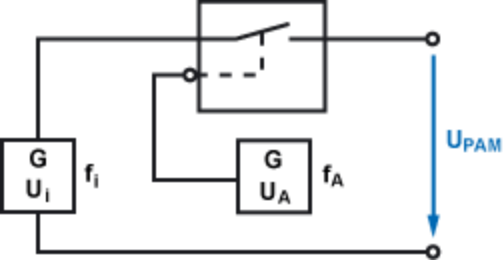
\includegraphics[scale=0.5]{PAM.png}\\
Die Erzeugung des PAM-Signals erfolgt über einen Analogschalter, der von einem Rechteckgenerator (fA) gesteuert wird. Dieser erzeugt das Trägersignal,
das aus schmalen sich periodisch wiederholenden Rechteckimpulsen besteht. Der Analogschalter öffnet und schließt entsprechend der Frequenz $f_A$ der Rechteckimpulse. 
Das PAM-Signal ist also immer nur ein Teilstück des Informationssignals. Man spricht bei diesem Vorgang von einer Abtastung. Deshalb wird die Frequenz $f_A$ auch Abtastfrequenz genannt.\\
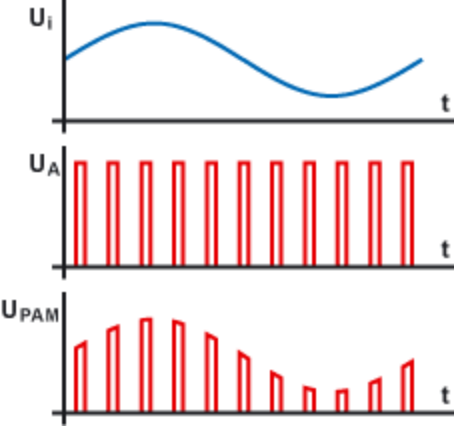
\includegraphics[scale=0.5]{PAM2.png}\\

Bei der Digitalisierung von Audiosignalen wird häufig die PAM verwendet. Zum Beispiel wird die bis 3,4 kHz begrenzten Sprachsignale bei der
ISDN-Telefonie mit 8 kHz abgetastet. Das normale Audiosignal, das bis 20 kHz reicht, wird mit 44,1 kHz abgetastet.
Grundsätzlich werden vor der Abtastung alle Frequenzen oberhalb der halben Abtastfrequenz durch einen Tiefpass (Anti-Aliasing-Filter) entfernt. 
Das PAM-Signal gibt es sowohl als unipolare Variante, bei der die Signaleimpulse alle im positiven oder negativen Bereich liegen, als auch eine
bipolare Variante, bei der die Signalimpulse im positiven und im negativen Bereich liegen können. Hier ist das PAM-Signal als unipolares Signal dargestellt.
Durch die Abtastimpulse entsteht eine amplitudenmodulierte Impulsfolge. Innerhalb der Impulspausen können über ein Zeitmultiplexverfahren noch andere Signale übertragen werden.

\subsubsection{Abtasttheorem nach Shannon}
Das Abtasttheorem sagt aus, dass ein beliebiges Audiosignal auch dann noch übertragen werden kann, wenn nur Teile davon in regelmäßigen Abständen übertragen werden.
\begin{align}
 f_A &> 2 \cdot f_{i,max}
\end{align}
Voraussetzung dafür ist, dass die Abtastfrequenz $f_A$ mindestens doppelt so groß sein muss, wie die höchste zu übertragene Frequenz des Informationssignals. 
Ist die Abtastfrequenz zu klein bzw. die Informationsfrequenz $f_i$ zu groß, dann fällt das Informationssignal in das Abtastsignal. Im modulierten Signal 
wäre die Amplitude des Informationssignals nicht vorhanden und könnte bei der Demodulation nicht wieder hergestellt werden.

\subsubsection{Aliasing-Effekt}
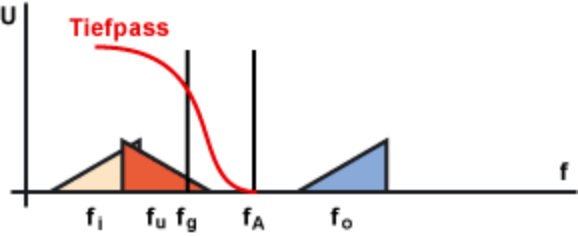
\includegraphics[scale=0.5]{Aliasing.png}\\
Wird das Abtasttheorem von Shannon nicht eingehalten, dann entsteht der Aliasing-Effekt. Das passiert immer dann, wenn sich das untere Seitenband $f_u$ mit der Informationsfrequenz 
$f_i$ überschneidet. Die Informationsfrequenz $f_i$ ist dann nicht mehr aus dem PAM-Signal rekonstruierbar. Deshalb muss die Abtastfrequenz $f_A$ mindestens doppelt so groß sein,
wie die zu übertragene Frequenz.


\subsubsection{PAM-Demodulation}
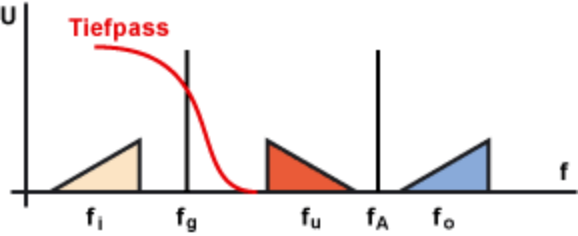
\includegraphics[scale=0.5]{PAM-demodulation.png}\\
Weil die ursprüngliche Informationsfrequenz $f_i$ im Frequenzspektrum des PAM-Signals enthalten ist, reicht für die Demodulation eines PAM-Signals ein Tiefpass aus.
Dieser muss aber eine hohe Güte aufweisen. Das bedeutet, der Tiefpass muss eine steile Flanke haben. Das ist besonders dann wichtig, wenn das untere Seitenband
nahe an das Informationssignal angrenzt.
\begin{align}
 f_g &= \frac{f_a}{2}
\end{align}
Die Grenzfrequenz des Tiefpasses liegt bei der Hälfte der Abtastfrequenz fA. Man bezeichnet diese Grenzfrequenz auch als Nyquistfrequenz.


\subsection{Pulscodemodulation}

\subsubsection{Eigenschaften der PCM-Technik}
 \begin{itemize}
 \item Die Signale lassen sich sehr leicht wieder regenerieren.
 \item Der Signal-Rausch-Abstand ist unabhängig von der Länge der Übertragungsstrecke.
 \item Die Signale weisen eine geringe Empfindlichkeit gegen Übersprechen auf.
 \item Die Signalübertragung ist auch bei alten, elektrisch ungünstigen Leitungen möglich.
 \item Die Signalübertragung erfolgt in Form binär kodierter Impulse.
 \item PCM ist hauptsächlich mit Halbleitern und integrierten Schaltkreisen realisierbar.
 \item Die Datenübermittlung und -verarbeitung erfolgt vollelektronisch.
 \item Hoher Aufwand durch Filterung, Abtastung, A/D-Wandlung und Multiplexing.
 \item Signalstörung durch den Quantisierungsfehler.
\end{itemize}






\subsection{Schritte der PCM-Technik}
\begin{itemize}
  \item Abtastung (PAM)
  \item Sample and Hold
  \item Quantisierung
  \item Codierung
\end{itemize}

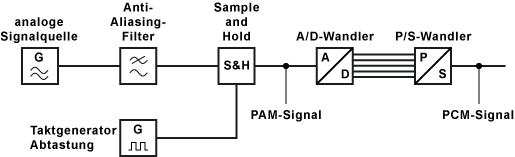
\includegraphics[scale=0.7]{PCM.png}\\

\subsubsection{Abtastung und Sample and Hold}
Die Abtastung erfolgt nach der PAM und dem Abtasttheorem von Shannon.Dabei wird das analoge Signal in 
ein PAM-Signal umgewandelt. Das PAM-Signal wird mit einer Sample-and-Hold-Stufe erzeugt. Dabei werden
die abgetasteten Impulse abgeflacht. Die ungleichmäßigen Impulse des PAM-Signal werden auf bestimmte Amplitudenstufen 
gebracht. Das Ausgangssignal ist dann ein zeitdiskretes stufenförmiges PAM-Signal.

\subsubsection{Quantisierung und Codierung}
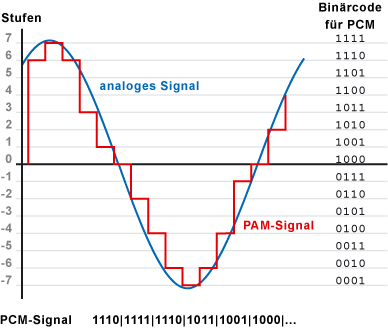
\includegraphics[scale=0.7]{Quantisierung.png}\\
Der wesentliche Bestandteil, um aus einem analogen Signal ein PCM-codiertes Signal zu wandeln, ist die Quantisierung. 
Die pulsamplitudenmodulierten Signale (PAM) werden in binäre Datenworte gewandelt. Dabei werden die einzelnen Amplitudenwerte 
(Spannungsstufen) entsprechenden Quantisierungsstufe und damit einem Binärcode zugeordnet. Der Binärcode wird dann als digitales 
Signal übertragen. Sowohl Sender und Empfänger wissen welcher Code welche Amplitude ausmacht.
Die Einteilung der Amplituden in Stufen wird als Quantisierung bezeichnet.

\subsubsection{PCM-Demodulation}
Die Demodulation eines pulscodemodulierten Signals entspricht genau umgekehrt der Erzeugung eines PAM-Signals.
Auf der Empfängerseite wird für jeden Quantisierungsintervall ein Signalwert zurückgewonnen, der den Mittelwert 
der Quantisierungsstufe entspricht. Dabei kommt es zu Abweichungen zum ursprünglichen Signal und Verzerrungen beim Ausgangssignal.

\subsubsection{Quantisierungsfehler}
Die Abtastung stellt nur eine Momentaufnahmen des analogen Signals dar. Diese Momentaufnahme muss über die Quantisierung einem Binärcode zugeordnet werden. 
Durch die nicht beliebig feine Quantisierung bei der Bildung des PCM-Signals entsteht der Quantisierungsfehler. Der eigentliche Spannungswert des Signals kann 
um maximal die Hälfte einer Quantisierungsstufe abweichen. Der Quantisierungsfehler macht sich als Verzerrung, dem Quantisierungsgeräusch, bemerkbar, 
das der Empfänger tatsächlich als Rauschen hören kann. Der Rauschanteil, der durch die A/D-Wandlung entsteht, nennt man Quantisierungsrauschen.
Um diese Verzerrungen zu umgehen, wird das Signal mit möglichst vielen Quantisierungsstufen aufgelöst und so der mögliche Quantisierungsfehler möglichst
vermieden. Je feiner die Abstufung, desto geringer fallen die Quantisierungsverzerrungen aus. Dabei steigt mit der Anzahl an Bits im Binärcode auch die
Datenmenge, die übertragen, gespeichert oder verarbeitet werden muss. Eine andere Maßnahme ist es, eine nichtlineare Quantisierung für die Digitalisierung
des Signals an die Anwendung anzupassen und so den Rauschabstand zu erhöhen und den Rauschanteil zu vermindern.

\subsection{Differential Pulscodemodulation}
Die Differential Pulse Code Modulation (DPCM) ist eine Erweiterung der Puls-Code-Modulation (PCM), und ist eine Vorstufe zur
Adaptive Differential Pulse Code Modulation (ADPCM). Bei DPCM werden Differenzwerte aufeinanderfolgender Abtastwerte gebildet, 
was bei Signalfolgen mit hoher Autokorrelation, wie es beispielsweise digitale Audiosignale sind, zu einer Datenreduktion führt.

\end{document}












